
%\documentclass[11pts,a4paper,amsmath,amssymb,floatfix]{article}%{report}%{book}
\documentclass[12pts,a4paper,amsmath,amssymb,floatfix]{article}%{report}%{book}
\usepackage{graphicx,wrapfig,pdfpages}% Include figure files
%\usepackage{dcolumn,enumerate}% Align table columns on decimal point
\usepackage{enumerate,enumitem}% Align table columns on decimal point
\usepackage{bm,dpfloat}% bold math
\usepackage[pdftex,bookmarks,colorlinks=true,urlcolor=rltblue,citecolor=blue]{hyperref}
\usepackage{amsfonts,amsmath,amssymb,stmaryrd,indentfirst}
\usepackage{times,psfrag}
\usepackage{natbib}
\usepackage{color}
\usepackage{units}
\usepackage{rotating}
\usepackage{multirow}


\usepackage{pifont}
\usepackage{subfigure}
\usepackage{subeqnarray}
\usepackage{ifthen}

\usepackage{supertabular}
\usepackage{moreverb}
\usepackage{listings}
\usepackage{palatino}
%\usepackage{doi}
\usepackage{longtable}
\usepackage{float}
\usepackage{perpage}
\MakeSorted{figure}
%\usepackage{pdflscape}


%\usepackage{booktabs}
%\newcommand{\ra}[1]{\renewcommand{\arraystretch}{#1}}


\definecolor{rltblue}{rgb}{0,0,0.75}


%\usepackage{natbib}
\usepackage{fancyhdr} %%%%
\pagestyle{fancy}%%%%
% with this we ensure that the chapter and section
% headings are in lowercase
%%%%\renewcommand{\chaptermark}[1]{\markboth{#1}{}}
\renewcommand{\sectionmark}[1]{\markright{\thesection\ #1}}
\fancyhf{} %delete the current section for header and footer
\fancyhead[LE,RO]{\bfseries\thepage}
\fancyhead[LO]{\bfseries\rightmark}
\fancyhead[RE]{\bfseries\leftmark}
\renewcommand{\headrulewidth}{0.5pt}
% make space for the rule
\fancypagestyle{plain}{%
\fancyhead{} %get rid of the headers on plain pages
\renewcommand{\headrulewidth}{0pt} % and the line
}

\def\newblock{\hskip .11em plus .33em minus .07em}
\usepackage{color}

%\usepackage{makeidx}
%\makeindex

\setlength\textwidth      {16.cm}
\setlength\textheight     {22.6cm}
\setlength\oddsidemargin  {-0.3cm}
\setlength\evensidemargin {0.3cm}

\setlength\headheight{14.49998pt} 
\setlength\topmargin{0.0cm}
\setlength\headsep{1.cm}
\setlength\footskip{1.cm}
\setlength\parskip{0pt}
\setlength\parindent{0pt}


%%%
%%% Headers and Footers
\lhead[] {\text{\small{EX3029 -- Chem. Thermodynamics}}} 
\rhead[] {{\text{\small{Assignment for Modules 4-5 (\today)}}}}
%\chead[\text{\small{\thepage}}]{\thepage}
%\chead[] {\text{\small{Session 2012/13}}} 
\lfoot[]{Dr Jeff Gomes}
%\rfoot[\today]{\today}
\rfoot[\text{\small{\thepage}}]{\thepage}
\renewcommand{\headrulewidth}{0.8pt}


%%%
%%% space between lines
%%%
\renewcommand{\baselinestretch}{1.5}

\newenvironment{VarDescription}[1]%
  {\begin{list}{}{\renewcommand{\makelabel}[1]{\textbf{##1:}\hfil}%
    \settowidth{\labelwidth}{\textbf{#1:}}%
    \setlength{\leftmargin}{\labelwidth}\addtolength{\leftmargin}{\labelsep}}}%
  {\end{list}}

%%%%%%%%%%%%%%%%%%%%%%%%%%%%%%%%%%%%%%%%%%%
%%%%%%                              %%%%%%%
%%%%%%      NOTATION SECTION        %%%%%%%
%%%%%%                              %%%%%%%
%%%%%%%%%%%%%%%%%%%%%%%%%%%%%%%%%%%%%%%%%%%

% Text abbreviations.
\newcommand{\ie}{{\em{i.e., }}}
\newcommand{\eg}{{\em{e.g., }}}
\newcommand{\cf}{{\em{cf., }}}
\newcommand{\wrt}{with respect to}
\newcommand{\lhs}{left hand side}
\newcommand{\rhs}{right hand side}
% Commands definining mathematical notation.

% This is for quantities which are physically vectors.
\renewcommand{\vec}[1]{{\mbox{\boldmath$#1$}}}
% Physical rank 2 tensors
\newcommand{\tensor}[1]{\overline{\overline{#1}}}
% This is for vectors formed of the value of a quantity at each node.
\newcommand{\dvec}[1]{\underline{#1}}
% This is for matrices in the discrete system.
\newcommand{\mat}[1]{\mathrm{#1}}


\DeclareMathOperator{\sgn}{sgn}
\newtheorem{thm}{Theorem}[section]
\newtheorem{lemma}[thm]{Lemma}

%\newcommand\qed{\hfill\mbox{$\Box$}}
\newcommand{\re}{{\mathrm{I}\hspace{-0.2em}\mathrm{R}}}
\newcommand{\inner}[2]{\langle#1,#2\rangle}
\renewcommand\leq{\leqslant}
\renewcommand\geq{\geqslant}
\renewcommand\le{\leqslant}
\renewcommand\ge{\geqslant}
\renewcommand\epsilon{\varepsilon}
\newcommand\eps{\varepsilon}
\renewcommand\phi{\varphi}
\newcommand{\bmF}{\vec{F}}
\newcommand{\bmphi}{\vec{\phi}}
\newcommand{\bmn}{\vec{n}}
\newcommand{\bmns}{{\textrm{\scriptsize{\boldmath $n$}}}}
\newcommand{\bmi}{\vec{i}}
\newcommand{\bmj}{\vec{j}}
\newcommand{\bmk}{\vec{k}}
\newcommand{\bmx}{\vec{x}}
\newcommand{\bmu}{\vec{u}}
\newcommand{\bmv}{\vec{v}}
\newcommand{\bmr}{\vec{r}}
\newcommand{\bma}{\vec{a}}
\newcommand{\bmg}{\vec{g}}
\newcommand{\bmU}{\vec{U}}
\newcommand{\bmI}{\vec{I}}
\newcommand{\bmq}{\vec{q}}
\newcommand{\bmT}{\vec{T}}
\newcommand{\bmM}{\vec{M}}
\newcommand{\bmtau}{\vec{\tau}}
\newcommand{\bmOmega}{\vec{\Omega}}
\newcommand{\pp}{\partial}
\newcommand{\kaptens}{\tensor{\kappa}}
\newcommand{\tautens}{\tensor{\tau}}
\newcommand{\sigtens}{\tensor{\sigma}}
\newcommand{\etens}{\tensor{\dot\epsilon}}
\newcommand{\ktens}{\tensor{k}}
\newcommand{\half}{{\textstyle \frac{1}{2}}}
\newcommand{\tote}{E}
\newcommand{\inte}{e}
\newcommand{\strt}{\dot\epsilon}
\newcommand{\modu}{|\bmu|}
% Derivatives
\renewcommand{\d}{\mathrm{d}}
\newcommand{\D}{\mathrm{D}}
\newcommand{\ddx}[2][x]{\frac{\d#2}{\d#1}}
\newcommand{\ddxx}[2][x]{\frac{\d^2#2}{\d#1^2}}
\newcommand{\ddt}[2][t]{\frac{\d#2}{\d#1}}
\newcommand{\ddtt}[2][t]{\frac{\d^2#2}{\d#1^2}}
\newcommand{\ppx}[2][x]{\frac{\partial#2}{\partial#1}}
\newcommand{\ppxx}[2][x]{\frac{\partial^2#2}{\partial#1^2}}
\newcommand{\ppt}[2][t]{\frac{\partial#2}{\partial#1}}
\newcommand{\pptt}[2][t]{\frac{\partial^2#2}{\partial#1^2}}
\newcommand{\DDx}[2][x]{\frac{\D#2}{\D#1}}
\newcommand{\DDxx}[2][x]{\frac{\D^2#2}{\D#1^2}}
\newcommand{\DDt}[2][t]{\frac{\D#2}{\D#1}}
\newcommand{\DDtt}[2][t]{\frac{\D^2#2}{\D#1^2}}
% Norms
\newcommand{\Ltwo}{\ensuremath{L_2} }
% Basis functions
\newcommand{\Qone}{\ensuremath{Q_1} }
\newcommand{\Qtwo}{\ensuremath{Q_2} }
\newcommand{\Qthree}{\ensuremath{Q_3} }
\newcommand{\QN}{\ensuremath{Q_N} }
\newcommand{\Pzero}{\ensuremath{P_0} }
\newcommand{\Pone}{\ensuremath{P_1} }
\newcommand{\Ptwo}{\ensuremath{P_2} }
\newcommand{\Pthree}{\ensuremath{P_3} }
\newcommand{\PN}{\ensuremath{P_N} }
\newcommand{\Poo}{\ensuremath{P_1P_1} }
\newcommand{\PoDGPt}{\ensuremath{P_{-1}P_2} }

\newcommand{\metric}{\tensor{M}}
\newcommand{\configureflag}[1]{\texttt{#1}}

% Units
\newcommand{\m}[1][]{\unit[#1]{m}}
\newcommand{\km}[1][]{\unit[#1]{km}}
\newcommand{\s}[1][]{\unit[#1]{s}}
\newcommand{\invs}[1][]{\unit[#1]{s}\ensuremath{^{-1}}}
\newcommand{\ms}[1][]{\unit[#1]{m\ensuremath{\,}s\ensuremath{^{-1}}}}
\newcommand{\mss}[1][]{\unit[#1]{m\ensuremath{\,}s\ensuremath{^{-2}}}}
\newcommand{\K}[1][]{\unit[#1]{K}}
\newcommand{\PSU}[1][]{\unit[#1]{PSU}}
\newcommand{\Pa}[1][]{\unit[#1]{Pa}}
\newcommand{\kg}[1][]{\unit[#1]{kg}}
\newcommand{\rads}[1][]{\unit[#1]{rad\ensuremath{\,}s\ensuremath{^{-1}}}}
\newcommand{\kgmm}[1][]{\unit[#1]{kg\ensuremath{\,}m\ensuremath{^{-2}}}}
\newcommand{\kgmmm}[1][]{\unit[#1]{kg\ensuremath{\,}m\ensuremath{^{-3}}}}
\newcommand{\Nmm}[1][]{\unit[#1]{N\ensuremath{\,}m\ensuremath{^{-2}}}}

% Dimensionless numbers
\newcommand{\dimensionless}[1]{\mathrm{#1}}
\renewcommand{\Re}{\dimensionless{Re}}
\newcommand{\Ro}{\dimensionless{Ro}}
\newcommand{\Fr}{\dimensionless{Fr}}
\newcommand{\Bu}{\dimensionless{Bu}}
\newcommand{\Ri}{\dimensionless{Ri}}
\renewcommand{\Pr}{\dimensionless{Pr}}
\newcommand{\Pe}{\dimensionless{Pe}}
\newcommand{\Ek}{\dimensionless{Ek}}
\newcommand{\Gr}{\dimensionless{Gr}}
\newcommand{\Ra}{\dimensionless{Ra}}
\newcommand{\Sh}{\dimensionless{Sh}}
\newcommand{\Sc}{\dimensionless{Sc}}


% Journals
\newcommand{\IJHMT}{{\it International Journal of Heat and Mass Transfer}}
\newcommand{\NED}{{\it Nuclear Engineering and Design}}
\newcommand{\ICHMT}{{\it International Communications in Heat and Mass Transfer}}
\newcommand{\NET}{{\it Nuclear Engineering and Technology}}
\newcommand{\HT}{{\it Heat Transfer}}   
\newcommand{\IJHT}{{\it International Journal for Heat Transfer}}

\newcommand{\frc}{\displaystyle\frac}
\newcommand{\red}{\textcolor{red}}
\newcommand{\blue}{\textcolor{blue}}
\newcommand{\green}{\textcolor{green}}
\newcommand{\purple}{\textcolor{purple}}
 
\newlist{ExList}{enumerate}{1}
\setlist[ExList,1]{label={\bf Example 1.} {\bf \arabic*}}

\newlist{ProbList}{enumerate}{1}
\setlist[ProbList,1]{label={\bf Problem 1.} {\bf \arabic*}}

%%%%%%%%%%%%%%%%%%%%%%%%%%%%%%%%%%%%%%%%%%%
%%%%%%                              %%%%%%%
%%%%%% END OF THE NOTATION SECTION  %%%%%%%
%%%%%%                              %%%%%%%
%%%%%%%%%%%%%%%%%%%%%%%%%%%%%%%%%%%%%%%%%%%


% Cause numbering of subsubsections. 
%\setcounter{secnumdepth}{8}
%\setcounter{tocdepth}{8}

\setcounter{secnumdepth}{4}%
\setcounter{tocdepth}{4}%


\begin{document}



\begin{enumerate}[label=\bfseries Problem \arabic*]

%%%
%%% Nguyen (Ex 5.3.1)  
%%%
\item\label{Example:1} Find the bubble point pressure and vapor composition for a liquid mixture of 41.2 mol$\%$ ethanol (1) and n-hexane (2) at 331 K. Given the Van Laar activity model equations:\hfill{\bf [15 Marks]}
\begin{displaymath}
\ln\gamma_{1} = \frc{A}{\left[1+\frc{A x_{1}}{B x_{2}}\right]^{2}}\;\;\;\; \ln\gamma_{2} = \frc{B}{\left[1+\frc{B x_{2}}{A x_{1}}\right]^{2}}\
\end{displaymath}
with A = 2.409 and B = 1.970. Also, the vapour pressure $\left(\text{with } P_{i}^{\text{sat}}\text{ in kPa and } T\text{ in K}\right)$ can be expressed as,
\begin{displaymath}
   \ln P_{1}^{\text{sat}} = 16.1952 - \frc{3423.53}{T-55.7152} \;\;\;\; \ln P_{2}^{\text{sat}} = 14.0568 - \frc{2825.42}{T-42.7089}
\end{displaymath}
%\begin{comment}
\bigskip

{\large{\bf Solution:}}{\it

   \begin{itemize}
      \item At 331 K,  $P_{1}^{\text{sat}}=$ 42.90 kPa and $P_{2}^{\text{sat}}=$ 70.54 kPa.~\hfill{\bf [2/15]}
      \item For the liquid solution with $x_{1}=0.412$ and $x_{2}=1-x_{1}=0.588$, the Van Laar equation,~\hfill{\bf [2/15]}
         \begin{eqnarray}
            \ln\gamma_{1} = \frc{2.409}{\left[1+\frc{2.409 x_{1}}{1.970 x_{2}}\right]^{2}} & \Longrightarrow & \gamma_{1} = 2.0111 \nonumber \\
            \ln\gamma_{2} = \frc{1.970}{\left[1+\frc{1.970 x_{1}}{2.409 x_{1}}\right]^{2}} & \Longrightarrow & \gamma_{2} = 1.5244 \nonumber
         \end{eqnarray}
      \item Partial pressure of ethanol and n-hexane are obtained from,~\hfill{\bf [2/15]}
         \begin{displaymath}
             P_{1} = x_{1}\gamma_{1}P_{1}^{\text{sat}} = 35.55 kPa,\;\;\;P_{2} = x_{2}\gamma_{2}P_{2}^{\text{sat}} = 63.22 kPa
         \end{displaymath}
      \item The bubble point pressure is~\hfill{\bf [3/15]}
         \begin{displaymath}
             {\bf P = P_{1} + P_{2} = 98.77 kPa}
         \end{displaymath}
      \item The composition of the vapour phase is~\hfill{\bf [6/15]}
         \begin{displaymath}
            {\bf y_{1} = \frc{P_{1}}{P} = 0.3599}\;\;\text{ and }\;\; {\bf y_{2} = \frc{P_{2}}{P} = 0.6401}
         \end{displaymath}
   \end{itemize}}
%\end{comment}
\clearpage

%%%
%%% Nguyen (Ex 5.3.2)  
%%%
\item\label{Example:2} Calculate the bubble point temperature and vapor composition for a liquid mixture of 1 mol$\%$ acetone (1) and water (2) at 101.3 KPa. Given the Wilson activity model:\hfill{\bf [15 Marks]}
   \begin{eqnarray}
       &&\ln\gamma_{1} = -\ln\left(x_{1}+x_{2}C_{12}\right) + x_{2}\left(\frc{C_{12}}{x_{1}+x_{2}C_{12}}-\frc{C_{21}}{x_{2}+x_{1}C_{21}}\right) \nonumber \\
       &&\ln\gamma_{2} = -\ln\left(x_{2}+x_{1}C_{21}\right) + x_{1}\left(\frc{C_{21}}{x_{2}+x_{1}C_{21}}-\frc{C_{12}}{x_{1}+x_{2}C_{12}}\right) \nonumber
   \end{eqnarray}
   with $C_{12}=$0.1173 and $C_{21}=$0.4227. Also, the vapour pressure $\left(\text{with } P_{i}^{\text{sat}}\text{ in kPa and } T\text{ in K}\right)$ is given by,
\begin{displaymath}
   \ln P_{1}^{\text{sat}} = 14.71712 - \frc{2975.95}{T-34.5228} \;\;\;\; \ln P_{2}^{\text{sat}} = 16.5362 - \frc{3985.44}{T-38.9974}
\end{displaymath}

%\begin{comment}
\bigskip

{\large{\bf Solution:}}{\it

   \begin{itemize}
      \item Since the vapour mole fractions are unknown, we should start from the main composition constraint, $\sum\limits_{i=1}^{2}y_{i} = 1$.  
      \item Replacing $y_{i}=x_{i}\gamma_{i}P_{i}^{\text{sat}}/P$,~\hfill{\bf [2/15]}
         \begin{displaymath}
            x_{1}\gamma_{1}P_{1}^{\text{sat}} + x_{2}\gamma_{2}P_{2}^{\text{sat}} = P
         \end{displaymath}
      \item For $x_{1} =$ 0.01, $x_{2} =$ 0.99, $C_{12} =$ 0.1173 and $C_{21} =$ 0.4227 $\Longrightarrow$ $\gamma_{1} =$ 13.0695 and $\gamma_{2} =$ 1.0007~\hfill{\bf [2/15]}
      \item With these numerical values, we can replace into the equation above,
         \begin{displaymath}
            (0.01)(13.0695)\exp\left[14.71712 - \frc{2975.95}{T-34.5228}\right] + (0.99)(1.000)\exp\left[16.5362 - \frc{3985.44}{T-38.9974}\right] =  101.3
         \end{displaymath}
         Resulting in {\bf $T=$ 361.71 K} -- the bubble point temperature of this acetone-water mixture.~\hfill{\bf [6/15]}
      \item At this temperature, the saturation pressure of acetone and water are $P_{1}^{\text{sat}}=$ 276.32 kPa and $P_{2}^{\text{sat}}=$ 65.78 kPa, respectively.~\hfill{\bf [2/15]}
      \item The vapour composition is~\hfill{\bf [3/15]}
         \begin{displaymath}
             \mathbf{y_{1} =\frc{x_{1}\gamma_{1}P_{1}^{\text{sat}}}{P} = 0.3565}\;\;\;\text{ and }\;\;\;\; \mathbf{y_{2} = 0.6435}
         \end{displaymath} 
   \end{itemize}}
\clearpage
%\end{comment}

%%%
%%% Nguyen (Ex 4.2.2)  
%%%
\item\label{Example:3} Fugacity and chemical potential of a fluid are related through the following differential equation,
      \begin{displaymath}
           d\mu = RTd\left(\ln f\right) = VdP,
      \end{displaymath}
      where $V$ is the molar volume.
      \begin{enumerate}
        \item Demonstrate that the van der Waals equation of state (vdW EOS),
               \begin{displaymath}
                  P = \frc{RT}{V-b} - \frc{a}{V^{2}},
               \end{displaymath}
               can be expressed as a cubic polynomial on $Z$,
               \begin{displaymath}
                   Z^{3}-\left(1+B\right)Z^{2} + AZ -AB = 0
               \end{displaymath}
               where $A= \frc{aP}{\left(RT\right)^{2}}$ and $B = \frc{bP}{RT}$.\hfill{\bf [15 Marks]}

        \item Show that the fugacity of a fluid represented by the vdW EOS can be calculated from the following equation
           \begin{displaymath}
             \ln\left(\frc{f}{P}\right) = -\ln\left(1-\frc{b}{V}\right) - \frc{a}{RTV} - \ln Z + \left(Z - 1\right),
           \end{displaymath}
           where $Z$ is the compressibility factor.\hfill{\bf [15 Marks]}
        \item Determine the fugacity of gaseous CO$_{2}$ at 310K and 1.4$\times$10$^{6}$ Pa using the vdW  EOS,
               \begin{displaymath}
                  P = \frc{RT}{V-b} - \frc{a}{V^{2}},
               \end{displaymath}
               Given: $a=$ 0.3658 Pa.m$^{6}$/gmol$^{2}$ and $b=$ 4.286$\times$10$^{-5}$ m$^{3}$/gmol.  \\
{\bf Hint:} Solving the vdW EOS leads to a polynomial of order 3. Use the largest real root of the polynomial to represent the gaseous phase.\hfill{\bf [15 Marks]}
     \end{enumerate}

%\begin{comment}
\bigskip 

{\bf Solution:}{\it 
\begin{enumerate}
% (a)
   \item The vdW EOS can be manipulated to obtain a non-linear equation in $Z$,~\hfill{\bf [4/15]}
        \begin{eqnarray}
           && P = \frc{RT}{V-b} - \frc{a}{V^{2}} \hspace{1cm} \red{\times \frc{V}{RT} }  \nonumber \\
           && \frc{PV}{RT} = \frc{V}{V-b} - \frc{a}{RTV} \Longrightarrow Z=\frc{1}{1- b/V} - \frc{a}{RTV}. \nonumber
        \end{eqnarray}
        As $V=\frc{ZRT}{P}$,~\hfill{\bf [2/15]}
        \begin{displaymath}
          Z = \frc{1}{1-\frc{bP}{ZRT}} - \frc{aP}{Z\left(RT\right)^{2}}.
        \end{displaymath}
        Defining $B=\frc{bP}{RT}$ and $A=\frc{aP}{(RT)^{2}}$, and substituting in the equation above,~\hfill{\bf [4/15]}
        \begin{displaymath}
           Z = \frc{1}{1-\frc{B}{Z}}-\frc{A}{Z}.
        \end{displaymath}
        Now rearranging into a polynomial format,~\hfill{\bf [5/15]}
        \begin{equation}
           Z^{3}-\left(1+B\right)Z^{2} + AZ -AB = 0.
         \label{example3:cubicZ} 
        \end{equation}
% (b)
   \item From the definition of fugacity, 
      \begin{equation}
           d\mu = RTd\left(\ln f\right) = VdP,\label{example3:eqn1}
      \end{equation}
       as the vdW EOS is explicitly expressed in terms of $P$, it is more convenient to rearrange Eqn.~\ref{example3:eqn1} to ensure that the $VdP$ term is easily integrated. For the ideal gas, Eqn.~\ref{example3:eqn1} can be rewritten as,~\hfill{\bf [1/15]}
      \begin{equation}
           RTd\left(\ln P\right) = VdP = \frc{RT}{P}dP.\label{example3:eqn2}
      \end{equation}
      Now subtracting Eqn.~\ref{example3:eqn2} from Eqn.~\ref{example3:eqn1},
      \begin{displaymath}
           RTd\left[\ln\left(\frc{f}{P}\right)\right] = \left(V-\frc{RT}{P}\right)dP, 
      \end{displaymath}
      and integrating from $0$ to $P$,~\hfill{\bf [2/15]}
      \begin{eqnarray}
           && RT\int\limits_{1}^{f/P}d\left[\ln\left(\frc{f}{P}\right)\right] = \int\limits_{0}^{P}\left(V-\frc{RT}{P}\right)dP \nonumber \\
           && \ln\left(\frc{f}{P}\right) = \frc{1}{RT} \int\limits_{0}^{P}\left(V-\frc{RT}{P}\right)dP.\label{example3:eqn3}
      \end{eqnarray}
       We want to change the \underline{integrating variable} from $P$ to $V$,~\hfill{\bf [1/15]}
      \begin{displaymath}
         d(PV) = PdV + VdP \Longrightarrow dP = \frc{1}{V}d(PV) - \frc{P}{V}dV;
      \end{displaymath}
      And using the definition of compressibiity factor, $Z=\frc{PV}{RT}$,
       \begin{displaymath}
          d(PV) = RT dZ \Longrightarrow dP = \frc{RT}{V}dZ - \frc{P}{V}dV = \frc{P}{Z}dZ - \frc{P}{V}dV;
       \end{displaymath}
      Now, replacing $dP$ in Eqn.~\ref{example3:eqn3}
       \begin{equation}
          \ln\left(\frc{f}{P}\right) = \frc{1}{RT} \int\limits_{V=\infty}^{V}\left(V-\frc{RT}{P}\right)\left(\frc{P}{Z}dZ-\frc{P}{V}dV\right)\label{example3:eqn4};
       \end{equation}
       And expanding the r.h.s., 
       \begin{equation}
          \ln\left(\frc{f}{P}\right) = \frc{1}{RT} \int\limits_{V=\infty}^{V}\left(\frc{RT}{V}-P\right)dV + \frc{1}{RT}\int\limits_{Z=1}^{Z}\left(\frc{PV}{Z}-\frc{RT}{Z}\right)dZ;\label{example3:eqn5}
       \end{equation}
        Integrating the second term of the r.h.s. of Eqn.~\ref{example3:eqn5},
       \begin{displaymath}
           \frc{1}{RT}\int\limits_{Z=1}^{Z}\left(\frc{PV}{Z}-\frc{RT}{Z}\right)dZ = \int\limits_{1}^{Z}\left(\frc{PV}{RT}\frc{1}{Z}-\frc{1}{Z}\right)dZ = \int\limits_{1}^{Z}\left(1 -\frc{1}{Z}\right)dZ = \left.\left(Z - \ln Z\right)\right|_{1}^{Z} = Z- \ln Z - 1
       \end{displaymath}
        Therefore,~\hfill{\bf [4/15]}
       \begin{equation}
          \ln\left(\frc{f}{P}\right) = \frc{1}{RT} \int\limits_{V=\infty}^{V}\left(\frc{RT}{V}-P\right)dV - \ln Z + \left(Z - 1\right);\label{example3:eqn6}
       \end{equation}
       Equation~\ref{example3:eqn6} is general equation for fugacity as function of molar volume and compressibility factor, and is valid for any real gas. The problem requires that we use the vdW EOS, therefore we need to manipulate it in order to be able to integrate with respect to V,~\hfill{\bf [3/15]}
        \begin{displaymath}
            P = \frc{RT}{V-b} - \frc{a}{V^{2}} \Longleftrightarrow \frc{RT}{V}-P = \frc{RT}{V}-\frc{RT}{V-b}+\frc{a}{V^{2}}
        \end{displaymath}
        \begin{eqnarray}
           \frc{1}{RT}\int\limits_{V=\infty}^{V}\left(\frc{RT}{V}-P\right)dV &=& \int\limits_{V=\infty}^{V}\frc{dV}{V} - \int\limits_{V=\infty}^{V} \frc{dV}{V-b} + \int\limits_{V=\infty}^{V} \frc{adV}{RTV^{2}} \nonumber \\
           &=& \left.\ln\frc{V}{V-b}\right|_{V^{\infty}}^{V} - \left.\frc{a}{RTV}\right|_{V^{\infty}}^{V} \nonumber \\
           &=& \ln\frc{V}{V-b} - \ln\frc{V^{\infty}}{V^{\infty}-b} - \left( \frc{a}{RTV} - \frc{a}{RTV^{\infty}}\right) \nonumber \\
           & & \blue{\left(\text{ as } \ln\frc{\infty}{\infty} = 0\;\;\; \text{ and } \frc{1}{\infty} \approx 0\right)} \nonumber \\ 
           &=& -\ln\frc{V-b}{V} - \frc{a}{RTV} = -\ln\left(1-\frc{b}{V}\right) - \frc{a}{RTV}; \nonumber
        \end{eqnarray}
        Therefore, replacing in Eqn.~\ref{example3:eqn6} 
        \begin{equation}
           \mathbf{\ln\left(\frc{f}{P}\right) = -\ln\left(1-\frc{b}{V}\right) - \frc{a}{RTV} - \ln Z + \left(Z - 1\right);}\label{example3:eqn7}
        \end{equation}
        this is the fugacity equation for the vdW EOS model.~\hfill{\bf [4/15]}
% (c)
   \item Using the recently defined $A$ and $B$ into Eqn.~\ref{example3:eqn7},~\hfill{\bf [3/15]}
           \begin{equation}
              \ln\left(\frc{f}{P}\right) = \left(Z-1\right) -\frc{A}{Z}-\ln\left(Z-B\right)\label{example3:eqn7b}
           \end{equation}
           Calculating $A$ and $B$:~\hfill{\bf [2/15]}
           \begin{eqnarray}
              A &=& \frc{aP}{\left(RT\right)^{2}}=0.3658\;\frc{Pa.m^{6}}{gmol} 1.4\times 10^{6}\;Pa \left(0.08314 \frc{bar.m^{3}}{kgmol.K}\cdot 310\;K\cdot \red{\frc{10^{5}\;Pa}{1\; bar} \cdot \frc{1\; kgmol}{1000\; gmol}}\right)^{-2} \nonumber \\
                &=& 7.7095\times 10^{-2} \nonumber \\
              B &=& \frc{bP}{RT} = 4.286\times 10^{-5} \frc{m^{3}}{gmol}\cdot \frc{1.4\times 10^{6}\;Pa}{0.08314 \frc{bar.m^{3}}{kgmol.K}\cdot 310\;K}\red{\cdot \frc{1\;bar}{10^{5}\;Pa}\cdot\frc{1000\; gmol}{1\; kgmol}} \nonumber \\
                &=& 2.3281\times 10^{-2} \nonumber
           \end{eqnarray}
           The cubic equation (Eqn.~\ref{example3:cubicZ}) becomes ~\hfill{\bf [3/15]}
           \begin{displaymath}
              Z^{3} - 1.023281 Z^{2} + 7.7095\times 10^{-2} Z - 1.7948\times 10^{-3} = 0
           \end{displaymath}
           Solving this polynomial of order 3 results in 3 roots:~\hfill{\bf [3/15]}
           \begin{eqnarray}
               && Z _{1} = 3.9844\times 10^{-2} \;\;\;\text{(smallest real root)} \nonumber\\
               && Z_{2} = 3.9844\times 10^{-2} - i \;\;\;\text{(root with imaginary component)} \nonumber\\
               && Z_{3} = 0.9436 \;\;\;\text{(largest real root)}\nonumber
           \end{eqnarray}
      Replacing $Z$ in Eqn.~\ref{example3:eqn7b}, leads to ${\bf f= 1.3250\times 10^{6}\text{ Pa}}$.~\hfill{\bf [4/15]}
   

\end{enumerate}}

\clearpage
%\end{comment}

%%%
%%% http://people.cst.cmich.edu/teckl1mm/PChemI/Chm351Ch7aF01.htm
%%%
\item\label{Example:4} The experimental value of the partial molar volume $\left(\text{cm}^{3}/\text{gmol}\right)$ of a aqueous solution of K$_{2}$SO$_{4}$ is given by
                \begin{displaymath}
                   \overline{V}_{A} = 32.280 + 18.216 m^{1/2},
                \end{displaymath} 
 where $m$ is the molality (= number of moles per kg of water) of the K$_{2}$SO$_{4}$ . 
     \begin{enumerate}%[(a)]
         \item Use the Gibbs-Duhem equation to derive an equation for the partial molar volume of water in the solution.\hfill{\bf [15 Marks]}
         \item Plot $\overline{V}_{i}\;\;\times m$, with $0.0\leq m\leq 0.1$. \hfill{\bf [10 Marks]}
     \end{enumerate}
    The molar volume of pure water at 298.15 K is 18.079 cm$^{3}$/gmol and the molar mass of pure water is 18 kg/kgmol.

%\begin{comment}
\bigskip

{\bf Solution:} {\it To ease the notation, let's take K$_{2}$SO$_{4}$: $A$ and Water: $w$

   \begin{enumerate}
%(a)
     \item The Gibbs-Duhem equation for the partial molar volumes can be expressed as,~\hfill{\bf [2/15]}
     \begin{displaymath}
        \sum\limits x_{i}d\overline{V}_{i} = x_{A} d\overline{V}_{A} + x_{w} d\overline{V}_{w} = 0,
     \end{displaymath}
     that after rearranging and integrating,~\hfill{\bf [2/15]}
     \begin{displaymath}
        \int\limits_{\overline{V}_{w}=V_{w}^{\circ}}^{\overline{V}_{w}}d\overline{V}_{w} = \overline{V}_{w} - V_{w}^{\circ} = -\int\frc{x_{A}}{x_{w}} d\overline{V}_{A},
     \end{displaymath}
     where $V_{w}^{\circ}$ is the molar volume of pure water at reference conditions (at $T=$ 25$^{\circ}$C).  We can change the integration variable from $\overline{V}_{A}$ to $m$,
      \begin{displaymath}
         \overline{V}_{A} = 32.280 + 18.216 m^{1/2} \rightarrow \frc{d\overline{V}_{A}}{dm} = \frc{1}{2}\cdot 18.216 m^{-1/2} 
      \end{displaymath} 
      Now, replacing it into the integral above,~\hfill{\bf [4/15]}
       \begin{eqnarray}
          && \overline{V}_{w} - V_{w}^{\circ} = -\int\frc{x_{A}}{x_{w}} \frc{1}{2}\cdot 18.216 m^{-1/2} dm \hspace{1cm} \red{\cdot\frc{n}{n}} \nonumber \\
          && \overline{V}_{w} - V_{w}^{\circ} = -\int\frc{n_{A}}{n_{w}} \frc{1}{2}\cdot 18.216 m^{-1/2} dm, \label{example4:eqn1}
       \end{eqnarray}
       where $n$ is the total number of moles in the solution.
\medskip
   
       From the definition of molality, i.e., number of moles of K$_{2}$SO$_{4}$ per kg of water,~\hfill{\bf [1/15]}
       \begin{displaymath}
           m = \frc{n_{A}}{n_{w}M_{w}} \Longrightarrow m\cdot M_{w} = \frc{n_{A}}{n_{w}},
       \end{displaymath}
       where $n_{A}$, $n_{w}$ are the number of moles of K$_{2}$SO$_{4}$ and water, respectively. $M_{w}$ is the molar mass of water.  Replacing in Eqn.~\ref{example4:eqn1}, ~\hfill{\bf [6/15]}
      \begin{eqnarray}
         \overline{V}_{w} - V_{w}^{\circ} &=& -\int\limits_{0}^{m} m\cdot M_{w} \frc{1}{2}\cdot 18.216 m^{-1/2} dm \nonumber \\
                                       &=& -9.108\; M_{w} \left. \frc{2}{3} m^{3/2}\right|_{0}^{m} \nonumber \\
         \blue{\left(\text{where }\right.}&& \blue{\left. M_{w} = 18 \frc{kg}{kgmol} = 0.018 \frc{kg}{gmol}\right)} \nonumber \\
         {\bf \overline{V}_{w}} &=& {\bf 18.079 - 0.1093 m^{3/2}} \nonumber 
      \end{eqnarray}
%(b)
  \item In order to plot $\overline{V}_{i}\;\;\times m$, with $0.0\leq m\leq 0.1$, we can use the defined equations above to set  up the table:~\hfill{\bf [10/10]}
        \begin{center}
          \begin{tabular}{|c | c c |}
            \hline
            ${\bf m (gmol/kg)}$ & ${\bf \overline{V}_{A}}$ & ${\bf \overline{V}_{w}}$ \\
            \hline
              0.00  & 32.2800 &  18.0790 \\
              0.05  & 36.6353 &  18.0778 \\
              0.10  & 38.0404 &  18.0755 \\
             \hline
          \end{tabular}
        \end{center}
          \begin{center}
              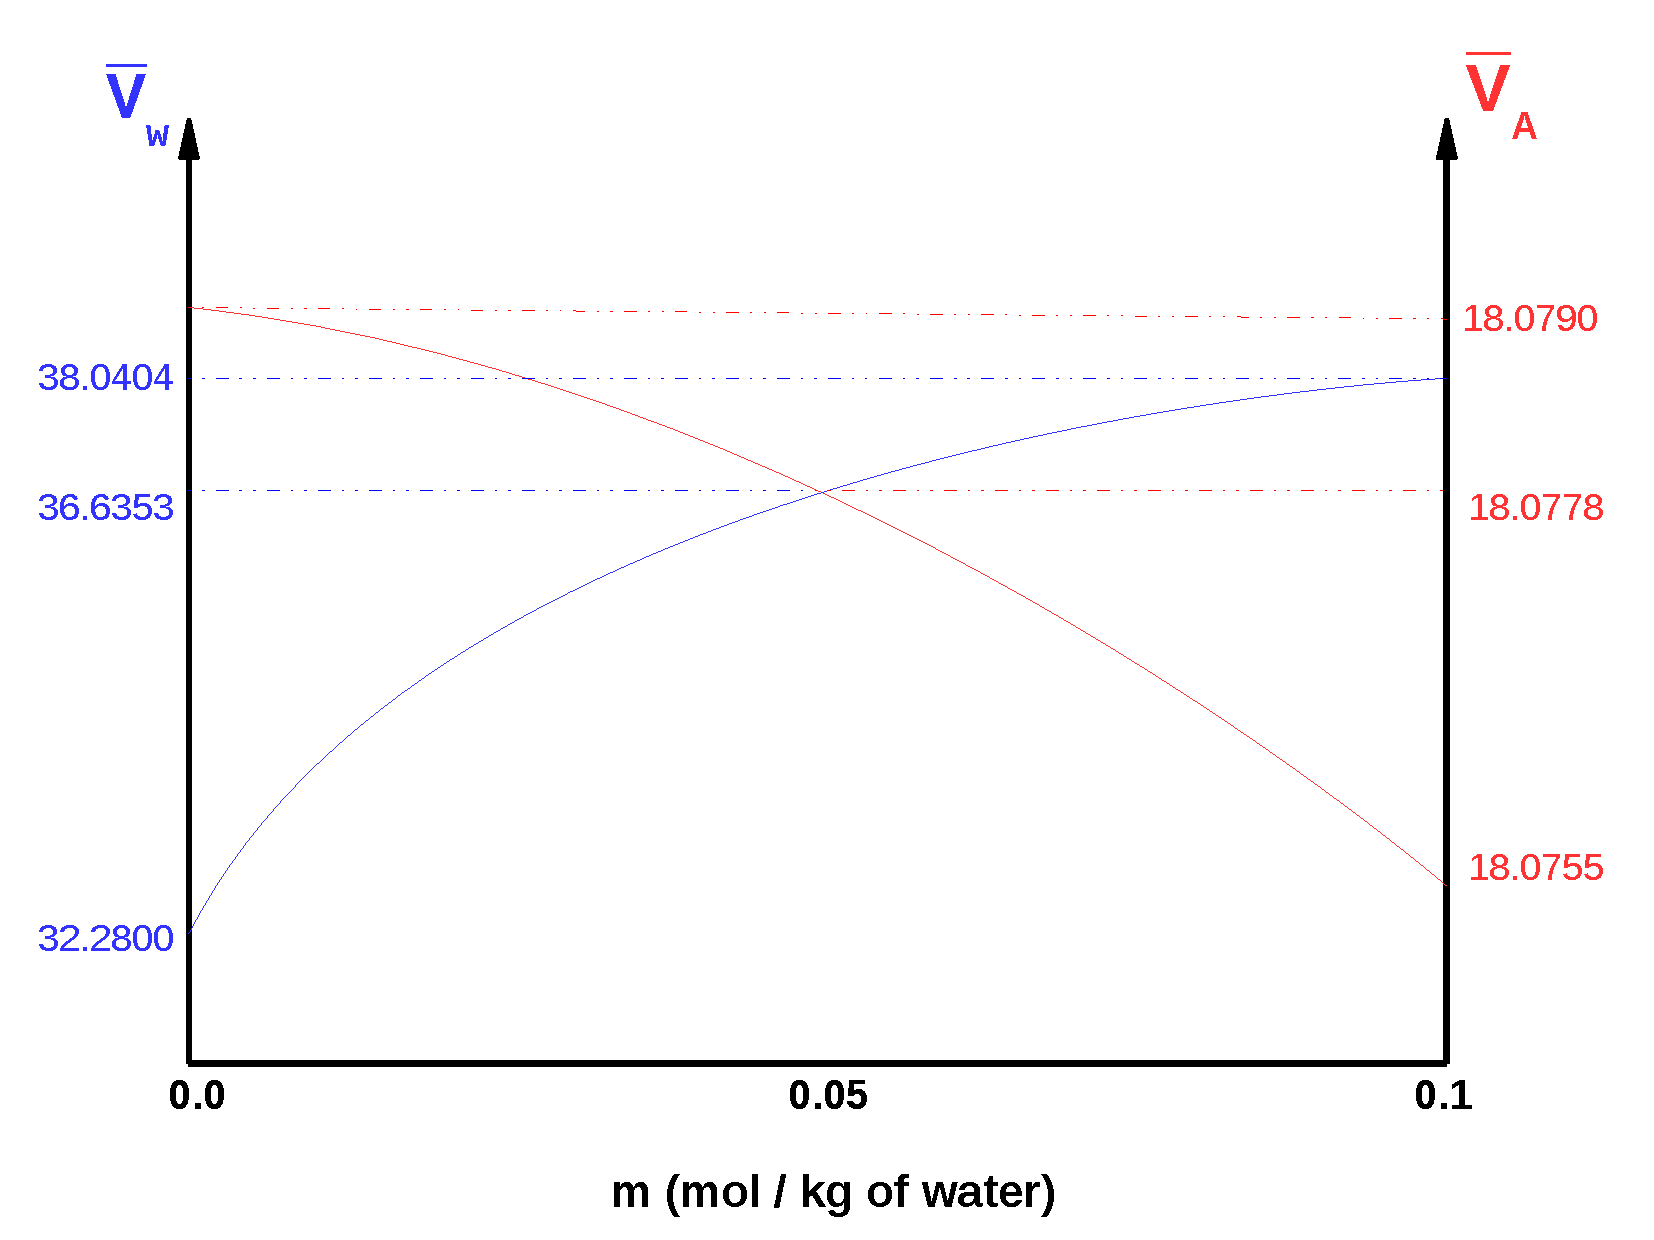
\includegraphics[width=0.75\columnwidth,clip]{./../Pics/Example04_Pic}
          \end{center}
\end{enumerate}
}
%\end{comment}
\end{enumerate} 
\begin{comment}
\clearpage

{\bf Deliverables:}
\begin{itemize}
\item Write a report containing the solutions for the problems 1-4 (including assumptions, derivations and plots). 
%
\item {\bf Prepare the report as \underline{PDF file} and submit it through {\it Turnitin} (with the appropriate plagiarism cover sheet) by Tuesday, December 15$^{th}$ 2015, 23:59 at the latest.}
%
\item Individual feedback will be provided on December 22$^{nd}$ 2015.
%
\item Penalties for late or non-submission are as follows:
\begin{enumerate}%[(a)]
\item Up to one week late, 2 CGS points deducted;
\item Up to two weeks late, 3 CGS point deducted;
\item More than two weeks late no marks awarded.
\end{enumerate}
If late or non-submission is due to medical or other circumstances out with your control you must submit a medical certificate or other formal evidence to the UG Office as soon as is practicable.% but no later than the end of Revision Week.


\item Note that the submitted work is part of the continuous assessment which will contribute 20$\%$ to your EX3029 mark.

\end{itemize}


%{
%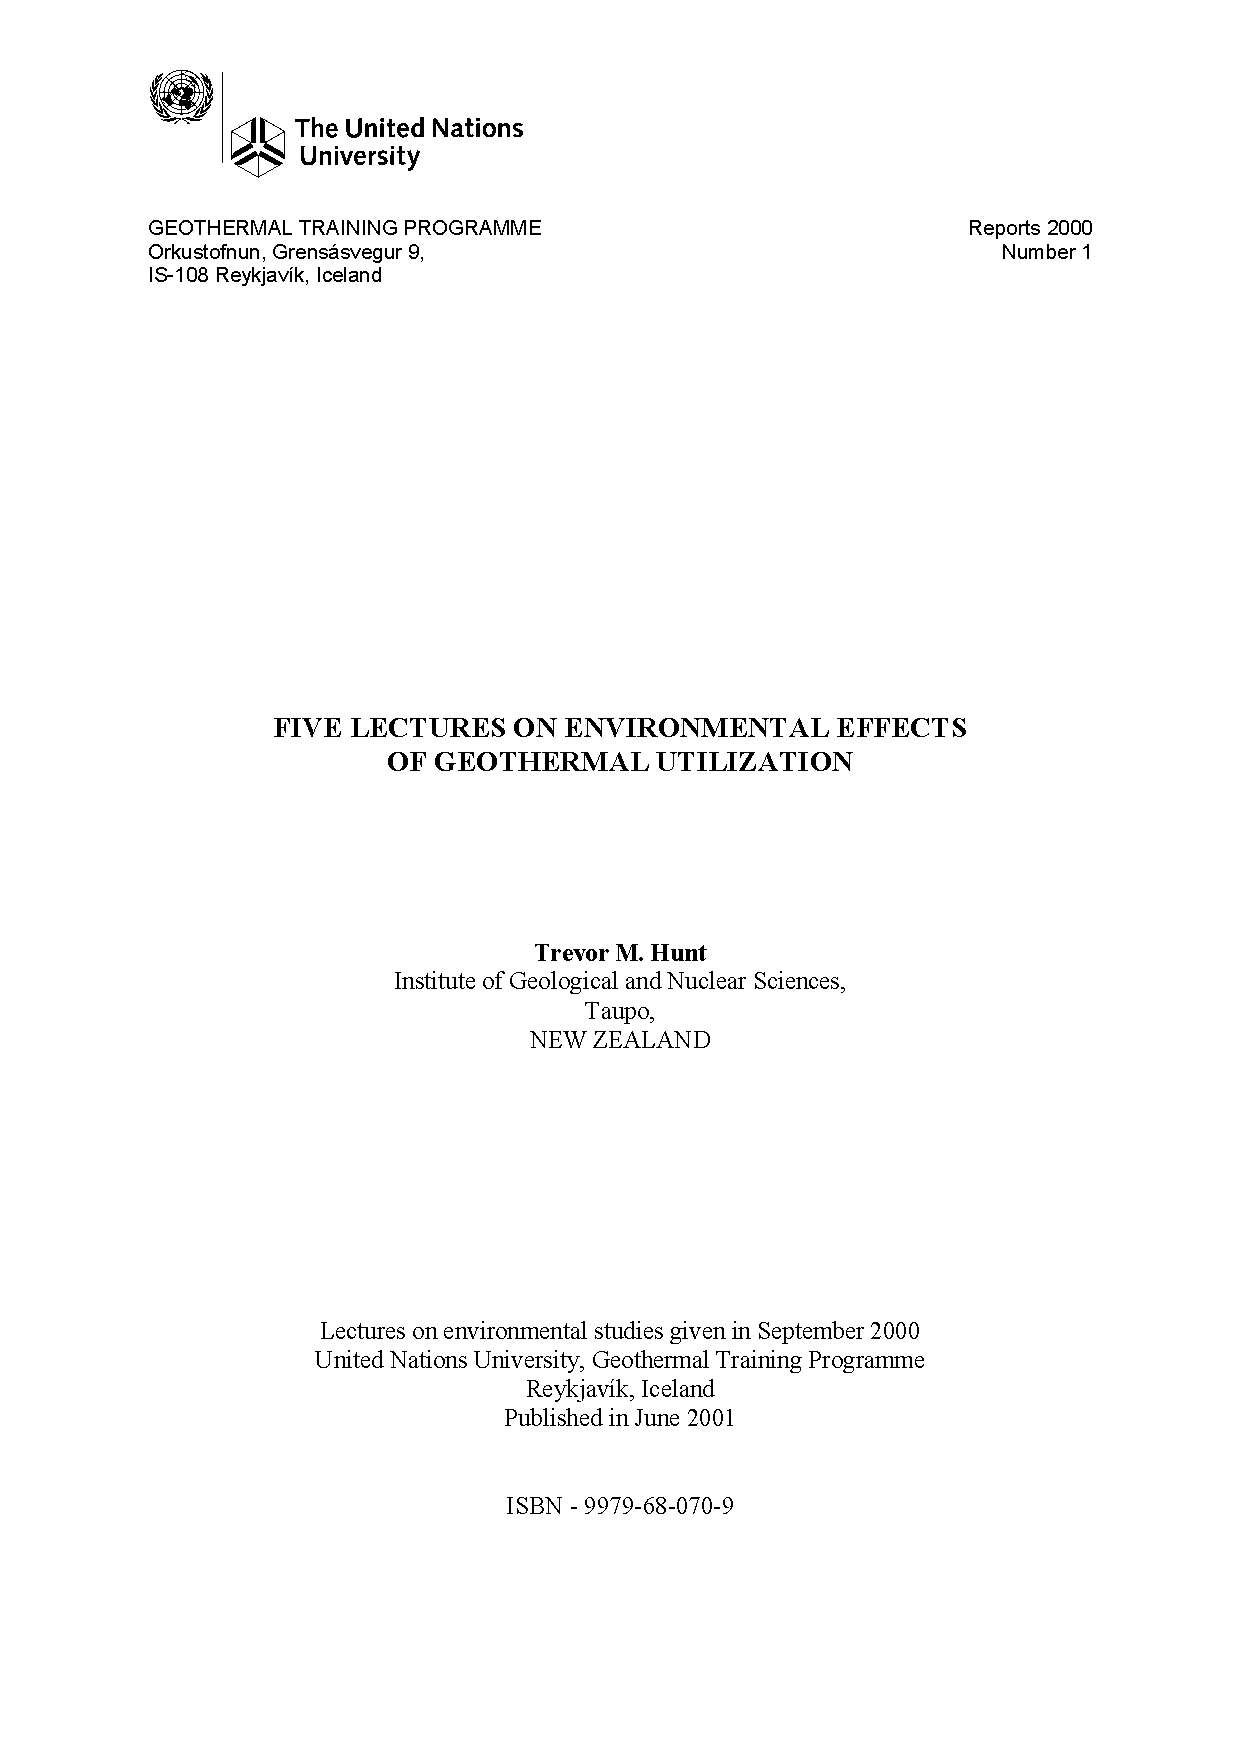
\includepdf[pages=-,fitpaper, angle=0]{./HuntSelect.pdf}
%}
\end{comment}
\end{document}
